\documentclass[12pt]{article}

\usepackage{a4wide,setspace} % spacing
\usepackage{graphicx} % inserting graphics
\usepackage[hang,small]{caption}

% Title
\title{\texttt{foxsisim-gui} Quickstart Guide}
\author{Robert Taylor\\\small{rlvtaylor@embarqmail.com}}
\date{\today}

\begin{document}
\maketitle
\newpage


%--------------------------------------%
\section*{Introduction}
%--------------------------------------%

The \texttt{foxsisim} python module is designed to simulate grazing incidence optics response to different light sources. The purpose of \texttt{foxsisim-gui} is to facilitate basic user operation with an easy to use GUI. Those familiar with the construction of optics modules such as the FOXSI telescope should find the user interface fairly intuitive. Nonetheless, this guide covers its basic use.


%--------------------------------------%
\section*{Module Settings}
%--------------------------------------%

A complete optic is created with the \texttt{foxsisim.module.Module} class. The first tab in the GUI, named \textit{Module}, facilitates module creation. There we see a table specifying \textit{shell radii} and \textit{angles} -- shells being the individual `tubes' within the module, each consisting of two mirrored \textit{segments} (see Figure \ref{fig:module}). 

\begin{figure}[ht]
\centering
	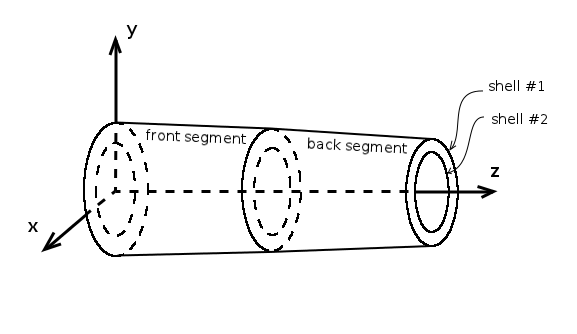
\includegraphics[scale=0.6]{figures/module.png}
\caption{\small A diagram demonstrating how a multishell optics module is represented within the \texttt{foxsisim} python code. The module base (aperture center) is located at the origin and the module is aligned along the $z$ axis. Rays must originate in the $-z$ region in order to pass through the module.}
\label{fig:module}
\end{figure}

\textit{Shell radius} refers to the distance from the $z$ axis to the place where the shell's two segments meet. \textit{Shell angle} refers to the angle between the front segment and the $z$ axis.

There are additional important settings below the table. \textit{Segment length} is self-explanatory, as are \textit{Detector Width} and \textit{Height}. \textit{Focal length} is the distance from the center of the module to the focal point. \textit{Detector Offset} is the distance along the $z$ axis by which the detector is offset from the focal point. A positive offset value means that the detector is farther from the module; negative means closer. The \textit{Detector Reso} is the pixel resolution of the detector.


%--------------------------------------%
\section*{Source Settings}
%--------------------------------------%

Next comes the \textit{Sources} tab. There we find a table that allows us to insert light sources of various \textit{types} into the system:
\begin{itemize}
\item \textbf{atinf}: the source is rectangular (\textit{Width} x \textit{Height}) and all rays travel in exactly the same direction (\textit{Normal})
\item \textbf{point}: all rays come from a single point (\textit{Center})
\item \textbf{nonpoint}: the source is rectangular (\textit{Width} x \textit{Height}) and rays can leave it in any direction
\end{itemize}

\textit{Center} is the location of the rectangular source. If the source is a point, then it is located at \textit{Center}. 

\textit{Normal} determines how a rectangular source is oriented (does not apply to point sources). Furthermore, if the source is \textbf{atinf}, \textit{Normal} is the direction in which rays will travel away from it.

\textit{Width} and \textit{Height} describe the dimension of the source's rectangular region. They do not apply to point sources.

Lastly, a source can be one of several \textit{colors}. If the detector catches rays from a source, then its color will be used to calculate detector pixel values.

%--------------------------------------%
\section*{Simulation}
%--------------------------------------%

The \textit{Simulation} tab allows us to simulate our module and light sources and provides some basic plotting functions. Once all module, detector, and source settings have been entered, we can simulate the system by entering the number of rays and pressing the \textit{Simulate} button. A simulation can easily be stopped and restarted without losing progress by using the \textit{Stop} button. However, if we wish to enter new module/detector/source settings, the \textit{Reset} button must be used.

A \textit{Detector Pixel Plot} is simply the captured image of the detector. The detector creates the image by storing the average color of rays that hit each pixel.

A \textit{Scatter Plot} displays the distribution of ray--detector collisions for one or more sources. Additionally, the \textit{Color Bounce Count} option tells \texttt{foxsisim} to color each point in the plot based on how many times it bounces within the module. Usually this color will be blue (two bounces) -- but under certain circumstances, points can be colored red (no bounces), green (one bounce), or black (more than two).



\end{document}


